\section{Introduction}
\begin{wrapfigure}{r}{0.4\textwidth}
    \centering
    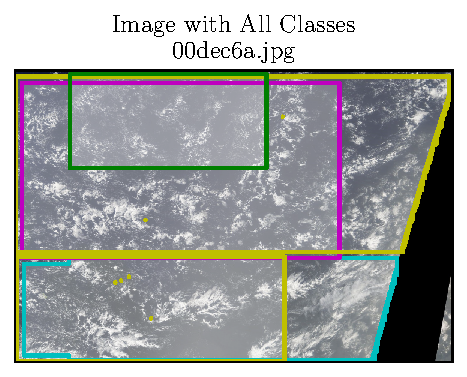
\includegraphics[width=3in]{figs/all_labels.pdf}
    \caption{A labeled training image showing all four types of clouds.}
    \label{fig:all_labels}
\end{wrapfigure}
%
This project follows the Kaggle Competition "\href{https://www.kaggle.com/competitions/understanding_cloud_organization/overview}{Understanding Clouds from Satellite Images}", hosted by the Max Planck Institute for Meteorology in 2019. The stated goal of the competition was to crowd source a way to better identify and label clouds in satellite images. The organizer provided a suite of training images, a \texttt{.csv} of the masks for each class in each image, and a suite of unlabeled test images. 
Provided by \href{https://worldview.earthdata.nasa.gov/}{NASA Worldview}, the \(2100 \times 1400\) pixel true-color images were acquired by two different polar-orbiting satellites, depicting shallow cumulus clouds in trade wind (ocean) regions. Despite being poorly represented in climate models, these types of clouds are thought to play a significant role in the Earth's radiation balance.

The organizers asked the competitors to build a model that could distinguish between four subjective patterns of clouds: \textbf{Sugar, Fish, Flower}, and \textbf{Gravel} \cite{rasp_CombiningCrowdsourcingDeep_2020, maxplanckinstituteformeteorology_UnderstandingCloudsSatellite_}; \cref{fig:all_labels} features a training image where all four classes are present. A team of scientists selected images of three different oceanic regions, then labeled them via group consensus. Some images feature discontinuities or artifacts related to observations being stitched together from multiple passes \cite{maxplanckinstituteformeteorology_UnderstandingCloudsSatellite_}.

Each team competing used the labeled training images to create some classification model with the ability to classify regions in new images, outputting creates a similar label map to the training labels provided. Each team is evaluated by applying their model to the test images and submitting a down-scaled label map to the Kaggle portal, at which point a DICE score is calculated as a proxy for performance (see \cref{eval}). The organizers reward the models with the best DICE score as the winner. 

\subsection*{Training Images}
\begin{figure}[htbp]
    \centering
    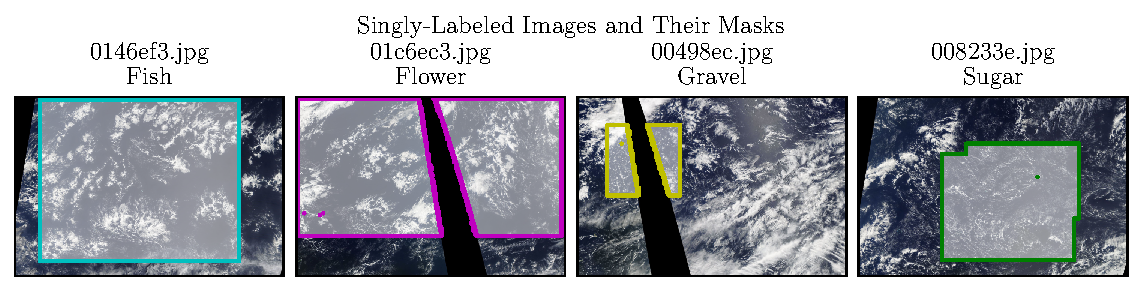
\includegraphics[width=\linewidth]{figs/single_labels.pdf}
    \caption{\textit{From left to right}: Images showing sugar, flower, fish, and gravel labels, respectively.}
    \label{fig:labeled_imgs}
\end{figure}
%
\begin{table}
    \centering
    \begin{tabular}{c|c}
    \hline
    Class  & Class Count \\ \hline
    Sugar  & 3,751       \\
    Gravel & 2,939       \\
    Fish   & 2,781       \\
    Flower & 2,365      
    \end{tabular}
    \quad
    \begin{tabular}{@{}c|c@{}}
    \toprule
    \begin{tabular}[c]{@{}c@{}}Number of\\ Classes Present\end{tabular} & \begin{tabular}[c]{@{}c@{}}Count of \\ Images\end{tabular} \\ \midrule
    1                                                                   & 1,348                                                        \\
    2                                                                   & 2,372                                                        \\
    3                                                                   & 1,348                                                        \\
    4                                                                   & 266                                                       
    \end{tabular}
    \caption{\textit{Left}: A table showing the number of labels available for each class in the training set. \textit{Right}: A table showing the number of images containing 1, 2, 3, and all 4 classes. }
    \label{tab:class_ct}
\end{table}
%
There are 5,546 training images provided, all of which depict clouds over water. Each image has some number of labeled regions of the four types of labels. \Cref{fig:all_labels} shows a rare training image with all types of clouds present, while \cref{fig:labeled_imgs} shows training images with only one class present in each image. 

A given image could contain any number of labeled regions belonging to each class, ranging from images with regions belonging to all four classes, to images with zero labeled regions. A summary of the number of classes per image is shown in \cref{tab:class_ct}.

\subsection*{Label Format}
The training labels are provided by the file \texttt{train.csv}, with four rows populated for each image. The first column specifies the image and the class, and the second column specifies the list of encoded pixels through run-length encoding (RLE). An example is shown in the table \cref{tab:RLE_ex}.
%
\begin{table}[h!]
    \centering
    \begin{tabular}{r|l}
    \multicolumn{1}{c|}{Image\_Label} & \multicolumn{1}{c}{EncodedPixels} \\ \hline
    \texttt{example\_img.jpg\_Fish}   & \texttt{1 3}        \\ \hline
    \texttt{example\_img.jpg\_Flower} & \texttt{10 8 22 40} \\ \hline
    \texttt{example\_img.jpg\_Gravel} &                                      \\ \hline
    \texttt{example\_img.jpg\_Sugar}  &                                     
    \end{tabular}
    \caption{An example how \texttt{example\_img.jpg} is labeled in the provided \texttt{train.csv}. The image has 3 pixels labeled as "Fish" starting at pixel 1, 8 pixels labeled as "Flower" starting at pixel 10, and 40 pixels labeled as "Flower" starting at pixel 22.}
    \label{tab:RLE_ex}
\end{table}

The RLE format references the one-indexed raveled pixel locations, starting from top to bottom and left to right. This means that the pixel \(1\) corresponds to the top-left corner, \((1,1)\), pixel \(2\) corresponds to the pixel to below pixel 1 at \((2, 1)\), etc. For each class within an image, the runs are listed in ascending order of the starting pixel. 
% 
\subsection*{Unlabeled Images and Evaluation} \label{eval}
There are 3,698 test images of the same resolution without labels. These test images are unlabeled and are only used to evaluate the classification model using the Dice (\(DSC\)) coefficient: 
%
\begin{equation*}
    DSC = \frac{2 | X \cap Y |}{|X| + |Y|}
\end{equation*}
%
Where \(X\) is the predicted set and \(Y\) is the ground truth. This would be unity for total agreement, and 0 for total disagreement. 

It should be noted that the submitted labels should reference the coordinates of the unlabeled images after they have been down sampled by a factor of four, giving labels to \(350 \times 525\) pixel images. Kaggle allows for late submissions of labels, giving a Dice coefficient for a submitted label list \cite{maxplanckinstituteformeteorology_UnderstandingCloudsSatellite_}. 